\subsubsection{Illustrative example}
\label{sec:illustrative example}
We consider a linear system with the following dynamics:
\begin{equation}
\label{eq:PointMass}
x_{k+1} = x_k + u_k
\end{equation}

The specification is 
\[\formula = \always_{[0,20]} \neg (x_k \in \text{Unsafe}) \land \eventually_{[0,20]} (x_k \in \text{Terminal})\]
with the sets $\text{Unsafe}=[-1,1]^2$ i.e. a hyper-cube in $\mathbb{R}^2$ with length 2, centered on the origin) and $\text{Terminal}=[2,2.5]^2$. 
The state space is $X=[-2.5,2.5]^2$, $U=[0.3,0.3]^2$, $\delta=1$, and we optimize for two different values of $\gamma$, $0.1$ and $0.001$. 
The initial point of the optimization is $x_0=[-2,-2]'$. 
The control cost is $l(x_k,u_k) = ||x_k||_{2}^2$, so that $\sum_kl(x_k,u_k)$ penalizes the length of the trajectory. Here, $hrz(\formula) = 21$.

\textbf{Optimization solver.}
We use Sequential Quadratic Programming (SQP) to solve the optimization problem $P_{\srob}$.
SQP solves constrained non-linear optimization problems, like $P_{\srob}$, by creating a sequence of quadratic approximations to the problem and solving these approximate problems.
SQP enjoys various convergence-to-(local)-optima properties, depending on the assumptions we place on the problem. 
See \cite[Section 2.9]{Polak97_Optim}.
For example, for SQP to converge to a strict local minimum (a minimum that is strictly smaller than any objective function value in an open neighborhood around it), it suffices that 
1) all constraint functions be twice Lipschitz continuously differentiable. 
In our case, this includes function $f$ in \eqref{eq:general ctrl obj}, and the problems we solve satisfy this requirement.
%We will need to assume that $f$ is twice Lipschitz continuously differentiable and that its gradient $f_u$ has maximum row rank.
And, 
2) at points in the search space that lie on the boundary of the inequality-feasible set (where the inequality constraints are satisfied with equality), there exists a search direction towards the interior of the feasible set that does not violate the equality constraints (the so-called Mangasarian-Fromowitz constraint qualification) \cite[Assumption 2.9.1]{Polak97_Optim}.
This is also true in our case since our equality constraints come from the dynamics and are always enforced for any $\mathbf{u}$.

\textbf{Solver initialization}.
To initialize SQP (i.e., give it a starting point for the optimization), we need an \textit{initial trajectory} that starts from $x_0$. We can obtain this initial trajectory:

 a) The standard way, by solving a feasibility linear program with constraints \eqref{eq:general ctrl dyn}-\eqref{eq:general ctrl U}. By definition, the solution to a feasibility program is a trajectory that simply satisfies the constraints without optimizing the objective. This is in general a computationally lightweight solution as the optimization being solved is a simple linear program.
 
 b) By randomly generating an input sequence (which respects the bounds on the input/states). Such a trajectory will be fast to generate and feasible w.r.t the dynamics but is unlikely to satisfy the specification on the system. 

Note, the initial trajectory is free to violate the specification (as it does in every example we study in this paper) and we only enforce that it needs to satisfy the dynamics and constraints of the system which we are controlling.

%In most cases, SQP solvers can also recover from infeasible starts, that is the initial trajectory can also violate the dynamics and constraints of the system, but at the cost of computation effort, hence we enforce the feasibility constraint on the initial trajectory.

\textbf{Comparison to BluSTL.}
We also compare the timing and robustness maximization performance for our method with BluSTL \cite{}. BluSTL has two modes of operation, \textit{boolean}: which aims at satisfying the specification (we set control cost to zero), and \textit{robust}: which uses a MILP encoding of robustness and attempts to maximize it (again we set control cost to zero). For a fair comparison of our method to BluSTL, we emulate the \textit{boolean} mode of BluSTL by terminating the optimization at the iteration of SQP where $\srob \geq \epsilon_{\text{Meyer}}$. The \textit{robust} operation is obtained by solving $P_{\srob}$ until SQP terminates (on a local minima, possibly global). Similar to the optimization cost of BluSTL, we set $\gamma=0$ in $P_{\srob}$ for both modes, i.e. no control cost. All methods are run in a \textit{one-shot} manner, that is a single optimization is solved at time step $0$ to get a trajectory with a length of $N$ time steps, where $hrz(\formula) = N$.


\textbf{Results}.
%Fig.~\ref{fig:toy control} shows the sets, initial trajectory (which is unsafe and has a robustness of $-1$), and two trajectories obtained by solving $P_{\srob}$ for two different values of $\gamma$ (with $\delta=0$). Both trajectories satisfy the specification $\formula$. Intuitively, the trajectories in Fig.\ref{fig:toy control} make sense, as for a higher value of $\gamma=0.1$ we get a shorter trajectory, which is closer to unsafe set, hence satisfies $\formula$ less robustly ($\rob_{\formula}=0.65$) and for a smaller value of $\gamma=0.001$ we get a longer trajectory with a higher robustness ($\rob_{\formula}=1.21$).
Fig. \ref{fig:toy control} shows the trajectories resulting from the SR-SQP and BluSTL in \textit{boolean} mode, SR-SQP in \textit{robust} mode, starting from the same initial state $[-2,-2]$. The last trajectory corresponds to SR-SQP in \textit{robust} mode with a non-zero cost for control corresponding to $\gamma=0.1$  in $P_{\srob}$ and a quadratic control cost function $l$. Note that BluSTL results in a trajectory that skirts the edge of the unsafe set and reaches a corner of the terminal set (resulting robustness is zero). SR-SQP (B) and SR-SQP (R) have a similar shape but SR-SQP (R) ends in the middle of the terminal set, resulting in a higher robustness as expected, while SR-SQP (B) terminates on reaching a positive robustness threshold as described above. SR-SQP (R,$\gamma=0.1$), takes into account the control cost and hence results in a trajectory of shorter length which trades of robustness ($0.236$ compared to $0.247$ for SR-SQP (R)) for control cost as is expected from the objective of $P_{\srob}$ in Eq. \ref{eq:general_ctrl}.


For detailed evaluation, we run 100 instances with the specification and dynamics of our illustrative example, with a random initial state $x_0 \in [-2.5,-1.5] \times [-2.5,2.5]$ for each instance. We also vary the formula horizon (and hence optimization length of the trajectory being optimized over) $N$ from $20$ to $200$ time-steps. Table \ref{tbl:time_performance_toy} shows the execution times for each method and the two modes of operation. All experiments were run on a machine with a quad-core Intel I5 3.2GHz processor with 24GB RAM, running MATLAB 2016b.


\begin{table}[tb]
\small
\begin{center}
\caption{{\small Runtimes (mean and standard, in seconds) for Smooth Operator (SR-SQP) and BluSTL (BlS) over 100 runs with random initial states and with different formula horizon lengths $N$. Here, (B) means \textit{boolean} mode and (R) means \textit{robust} mode of operation.}}
\vspace{-5pt}
\label{tbl:time_performance_toy}
\begin{tabular} {|c|c|c|c|c|}
	\hline
	N & BlS(B) & SR-SQP(B) & BlS(R) & SR-SQP(R) \\ \hline
	20 & $0.96 \pm 0.82$ &  $\mathbf{0.31 \pm 0.13}$  & NA & $3.30 \pm 1.25$ \\ \hline
	30 & $1.37 \pm 1.72$ &  $\mathbf{0.33 \pm 0.25}$  & NA & $5.85 \pm 2.74$\\ \hline
	40 & $3.86 \pm 5.10$ &  $\mathbf{0.60 \pm 0.29}$  & NA & $12.36 \pm 6.04$\\ \hline
	50 & $4.36 \pm 12.97$&  $\mathbf{0.74 \pm 0.30}$ & NA & $30.05 \pm 18.23$\\ \hline
	100& $16.77 \pm 27.84$ & $\mathbf{1.21 \pm 0.25}$ & NA & $69.70 \pm 13.16$ \\ \hline
	200& $53.88 \pm 14.18$& $\mathbf{4.19 \pm 1.18}$ & NA & $126.11 \pm 20.43$ \\ \hline
\end{tabular}	
\end{center}
\end{table}

\textbf{Analysis.}
As seen in table \ref{tbl:time_performance_toy}, our method is consistently faster than BluSTL for the \textit{boolean} mode, and also displays smaller variances in runtimes. For BluSTL in \textit{robust} mode, BluSTL could not finish a single instance of robustness maximization within 100 hours on both the machine used for running experiments as well as on a machine with 8 core Intel Xeon machine with 60GB RAM, leading us to believe that the problem formulation in BluSTL did not scale into a tractable MILP. Note, the problem solved here is very similar to the example used in \cite{Saha_acc16}, which uses another MILP based method to find satisfying trajectories. While the underlying dynamics and the machine on which evaluations are run are different, these results suggest that our run-times compare favourably with those in \cite{Saha_acc16}.

When in \textit{boolean} mode, BluSTL results in trajectories with zero robustness (as seen in fig. \ref{fig:toy control}), while our method results in trajectories with an average robustness of 0.10. Both methods satisfy $\formula$ in all 100 instances. In \textit{robust} mode, across all experiments, SR-SQP results in an average $\rob_{\formula}=0.247$ with a standard deviation of less than $0.005$. It is to be noted, that an upper bound on the maximum achievable $\rob_{\formula}$ is $0.25$, which can be achieved by trajectory reaching (in number of time steps $\leq N$) the point $[2.25,2.25]$ in the middle of the Terminal set while always avoiding the Unsafe set by a distance greater than $0.25$. This shows that for this problem, our method reaches very close to achieving the global optima of $\rob_{\formula}$. Also with this additional knowledge of the global optima upper bound, the SR-SQP method in \textit{robust} mode can be made a lot faster by specifying an exit condition based on a upper threshold of $\srob_{\formula}$ attained at any iteration of the SR-SQP method. While for brevity we do not include results with this additional stopping criteria, it was observed that for an upper bound value of $\srob_{\formula}=0.24$, an average speed up of about $4$-times was observed for $N=20$ and $2$-times for $N=200$ while resulting an average robustness value achieved of $\rob_{\formula} = 0.235$. This shows that with the iterative nature of SQP, we can trade-off performance for improved execution times.

\textbf{Note} that in BluSTL, atomic propositions in general have to be of the form $a'x\leq b$ (although absolute value and polynomials are also valid) since robustness is encoded as a MILP, which necessitates avoiding the signed distance function in dimensions greater than 1. This implies that atomic propositions in higher dimensions ($x\in \mathbb{R}^{n>1}$), $Hx \leq g$, have to be broken down into the conjunction of $n$ individual atomic propositions of the form $h_i'x \leq g_i$. This also restricts atomic propositions in BluSTL from involving sets like circles or ellipsoids. On the other hand, atomic propositions in our work can involve non-Polyhedron sets (e.g. ellipsoids or circles) and even non-convex sets since we do not avoid the signed distance function for higher dimensions.

\begin{figure}[t]
\centering
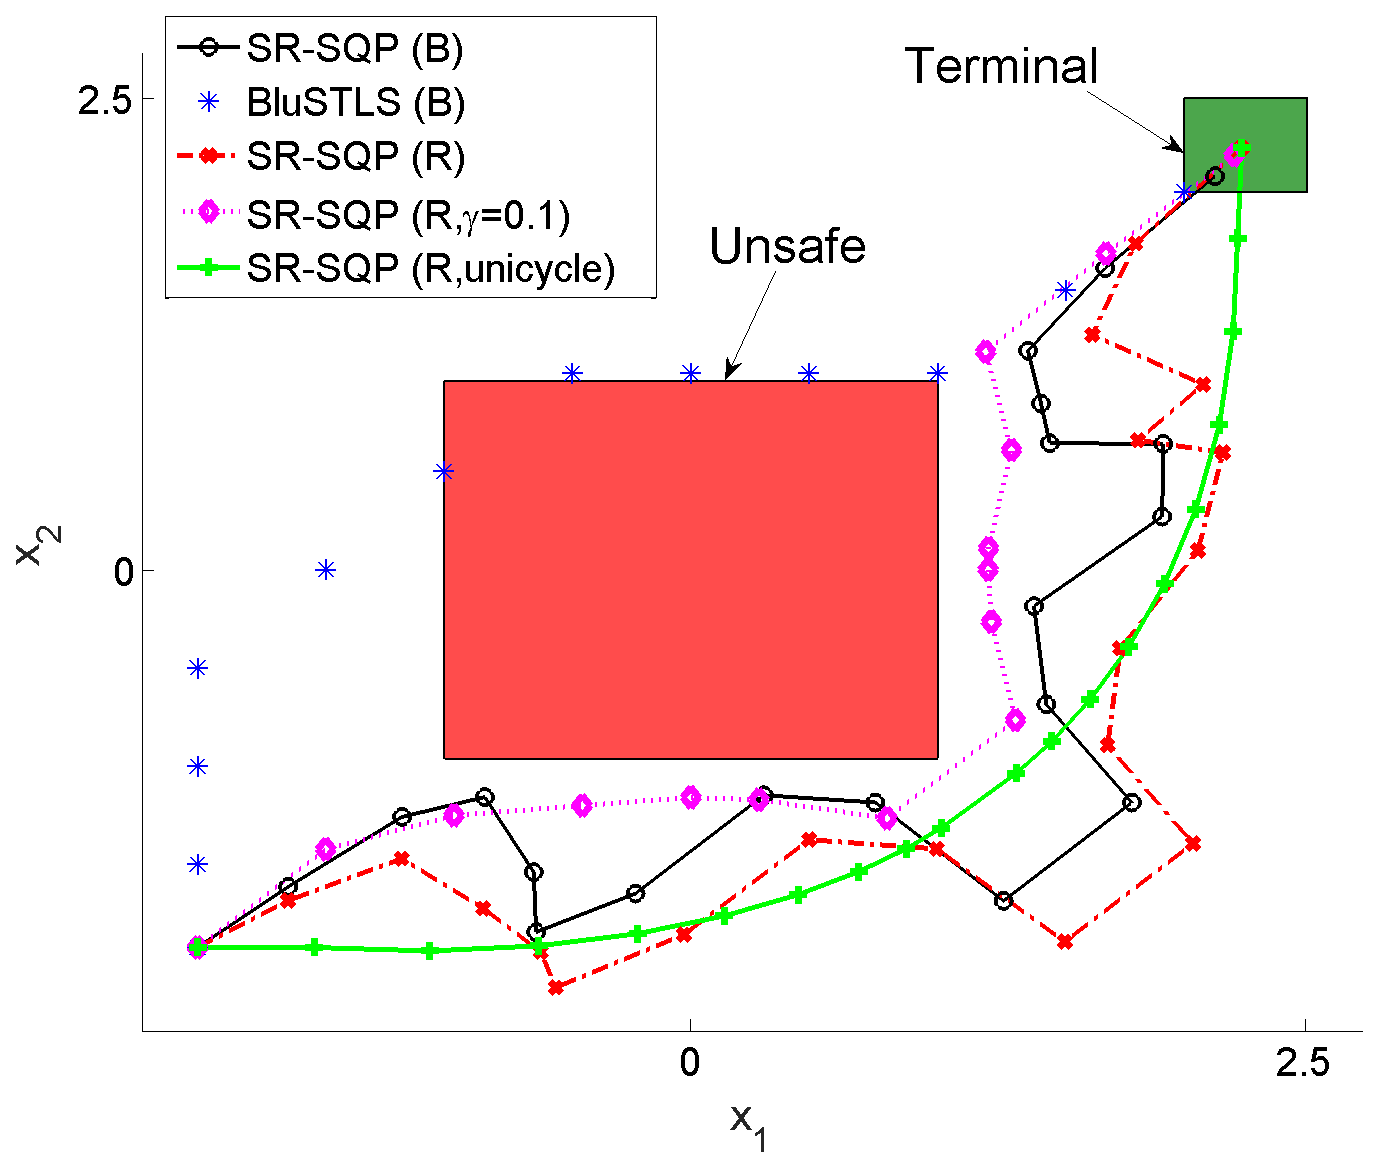
\includegraphics[width=0.49\textwidth]{figures/ToyExUni_scissored.pdf}
\vspace{-20pt}
\caption{{\small Trajectories for the illustrative example for SR-SQP and BluSTL. B, R refer to the \textit{Boolean} and \textit{Robust} mode of operation. Refer to the discussion in Sec. \ref{sec:illustrative example}}, Results for an explanation. Color in online version.}
\label{fig:toy control}
\vspace{-10pt}
\end{figure}